\section{Experiments}
\label{sec:exp}
\begin{table}[t]
    \centering
    \caption{Performance comparison with \textbf{GUI-Owl-1.5} series. \textbf{Avg.\,(\%)} denotes performance relative to the upper bound. Best and second-best results are shown in \textbf{bold} and \underline{underlined}, respectively.}
    \label{tab:main-combined}
    \resizebox{\textwidth}{!}{%
        \setlength{\tabcolsep}{6pt}%
        \renewcommand{\arraystretch}{0.92}%
        \begin{tabular}{l ccc ccc c}
            \toprule
            \multirow{2}{*}{\textbf{Method}} & \multicolumn{3}{c}{\textbf{Single-step (Accuracy)}} & \multicolumn{3}{c}{\textbf{Multi-step (Step~SR)}} & \multirow{2}{*}{\textbf{Avg.\,(\%)}} \\
            \cmidrule(lr){2-4}\cmidrule(lr){5-7}
            & SS-v2 & SS-Pro & MMBench-GUI & OmniGUI & Mind2Web & AndroidControl &  \\
            \midrule
            \rowcolor{headergray}\multicolumn{8}{c}{\textsc{GUI-Owl-1.5-8B: Upper Bound (100\% Tokens)}} \\
            GUI-Owl-1.5-8B & 93.79 & 70.34 & 82.64 & 52.45 & 52.90 & 60.41 & 100.0\% \\
            \rowcolor{headergray}\multicolumn{8}{c}{\textsc{Mild Budget (Single-step: $\keepr{=}10\%$ \,$||$\, Multi-step: $\keepc{=}50\%$, $\keeph{=}10\%$)}} \\
            Random & 33.81 & 6.14 & 18.53 & 43.16 & 35.13 & 58.82 & 52.2\% \\
            Uniform & 43.79 & 10.69 & 28.27 & 46.11 & 39.65 & 59.08 & 59.5\% \\
            DivPrune\pub{(CVPR25)\cite{alvar2025divprune}} & 51.97 & 13.98 & 31.61 & 45.76 & 40.70 & 58.83 & 62.5\% \\
            CDPruner\pub{(NeurIPS25)\cite{zhang2025cdpruner}} & 33.18 & 11.26 & 12.21 & 41.45 & 27.88 & 54.57 & 48.0\% \\
            VisPruner\pub{(ICCV25)\cite{zhang2025vispruner}} & 51.73 & 34.41 & \underline{42.35} & 46.11 & 44.45 & 59.25 & 70.9\% \\
            PruMerge+\pub{(ICCV25)\cite{shang2025prumerge}} & 40.49 & 19.80 & 30.47 & 46.50 & 41.53 & 59.28 & 62.2\% \\
            TRIM\pub{(COLING25)\cite{song2025trim}} & 36.24 & 3.29 & 25.24 & 45.84 & 41.20 & 56.86 & 55.5\% \\
            FastV\pub{(ECCV24)\cite{chen2024fastv}} & 52.04 & 28.53 & 40.21 & 46.89 & 43.12 & 59.11 & 68.9\% \\
            VisionTrim\pub{(ICLR26)\cite{yu2026visiontrim}} & 58.65 & \textbf{38.52} & 40.71 & 45.72 & 43.91 & 59.10 & \underline{72.4\%} \\
            ZOO-Prune\pub{(CVPR26)\cite{kim2026zooprune}} & 56.29 & 9.55 & 35.98 & \underline{48.17} & \underline{44.98} & 59.30 & 65.4\% \\
            PruneSID\pub{(ICLR26)\cite{fang2026prunesid}} & \underline{58.96} & 15.69 & 40.65 & 47.40 & 43.28 & \underline{59.52} & 67.5\% \\
            \rowcolor{rowblue}\textbf{\method{}} & \textbf{73.90} & \underline{37.63} & \textbf{50.47} & \textbf{48.91} & \textbf{45.52} & \textbf{60.20} & \textbf{78.7\%} \\
            \rowcolor{headergray}\multicolumn{8}{c}{\textsc{Tight Budget (Single-step: $\keepr{=}5\%$ \,$||$\, Multi-step: $\keepc{=}25\%$, $\keeph{=}5\%$)}} \\
            Random & 15.49 & 1.27 & 9.29 & 34.25 & 18.43 & 52.07 & 36.0\% \\
            Uniform & 21.38 & 3.04 & 12.24 & 38.96 & 20.61 & \underline{56.13} & 41.3\% \\
            DivPrune\pub{(CVPR25)\cite{alvar2025divprune}} & 25.71 & 3.86 & 14.11 & 37.17 & 24.29 & 54.75 & 42.9\% \\
            CDPruner\pub{(NeurIPS25)\cite{zhang2025cdpruner}} & 15.88 & 3.48 & 4.76 & 27.76 & 10.86 & 40.90 & 28.1\% \\
            VisPruner\pub{(ICCV25)\cite{zhang2025vispruner}} & 20.68 & 12.21 & 16.75 & 39.54 & \underline{30.67} & 54.93 & 47.3\% \\
            PruMerge+\pub{(ICCV25)\cite{shang2025prumerge}} & 17.85 & 5.88 & 12.19 & 36.98 & 23.45 & 54.01 & 41.1\% \\
            TRIM\pub{(COLING25)\cite{song2025trim}} & 15.88 & 0.44 & 9.85 & 34.37 & 23.01 & 47.17 & 36.1\% \\
            FastV\pub{(ECCV24)\cite{chen2024fastv}} & 28.38 & 11.83 & \underline{20.51} & 39.39 & 29.33 & 54.61 & 48.8\% \\
            VisionTrim\pub{(ICLR26)\cite{yu2026visiontrim}} & 25.86 & \underline{18.22} & 16.86 & 38.26 & 30.20 & 55.16 & \underline{49.2\%} \\
            ZOO-Prune\pub{(CVPR26)\cite{kim2026zooprune}} & 28.46 & 3.48 & 15.33 & 40.01 & 27.90 & 55.76 & 45.9\% \\
            PruneSID\pub{(ICLR26)\cite{fang2026prunesid}} & \underline{34.20} & 4.55 & 19.48 & \underline{40.09} & 27.57 & 55.46 & 47.8\% \\
            \rowcolor{rowblue}\textbf{\method{}} & \textbf{55.19} & \textbf{20.30} & \textbf{30.88} & \textbf{43.08} & \textbf{34.20} & \textbf{57.06} & \textbf{61.1\%} \\
            \rowcolor{headergray}\multicolumn{8}{c}{\textsc{GUI-Owl-1.5-2B: Upper Bound (100\% Tokens)}} \\
            GUI-Owl-1.5-2B & 90.49 & 57.94 & 71.84 & 39.70 & 44.23 & 57.93 & 100.0\% \\
            \rowcolor{headergray}\multicolumn{8}{c}{\textsc{Tight Budget (Single-step: $\keepr{=}5\%$ \,$||$\, Multi-step: $\keepc{=}25\%$, $\keeph{=}5\%$)}} \\
            Random & 14.54 & 1.71 & 8.35 & 24.77 & 16.21 & 47.43 & 35.3\% \\
            Uniform & 13.52 & 2.59 & 8.07 & 25.66 & 15.92 & 52.38 & 36.9\% \\
            DivPrune\pub{(CVPR25)\cite{alvar2025divprune}} & 18.00 & 2.28 & 8.57 & 26.52 & 20.52 & 50.30 & 39.3\% \\
            CDPruner\pub{(NeurIPS25)\cite{zhang2025cdpruner}} & \underline{22.17} & 2.66 & \underline{13.05} & 27.10 & 18.20 & 50.19 & 40.6\% \\
            VisPruner\pub{(ICCV25)\cite{zhang2025vispruner}} & 12.81 & 2.34 & 6.68 & 22.55 & 18.85 & 48.59 & 35.1\% \\
            PruMerge+\pub{(ICCV25)\cite{shang2025prumerge}} & 12.03 & 2.34 & 6.98 & 23.17 & 14.68 & 47.35 & 33.4\% \\
            TRIM\pub{(COLING25)\cite{song2025trim}} & 17.37 & 1.58 & 9.63 & 25.35 & 23.58 & 51.28 & 40.2\% \\
            FastV\pub{(ECCV24)\cite{chen2024fastv}} & 10.46 & \underline{6.58} & 7.57 & 25.51 & \textbf{27.62} & 51.71 & 41.6\% \\
            VisionTrim\pub{(ICLR26)\cite{yu2026visiontrim}} & 17.30 & 4.43 & 9.43 & 23.72 & 17.80 & 49.43 & 37.5\% \\
            ZOO-Prune\pub{(CVPR26)\cite{kim2026zooprune}} & 19.50 & 1.58 & 10.35 & 26.17 & 22.78 & 53.06 & 41.3\% \\
            PruneSID\pub{(ICLR26)\cite{fang2026prunesid}} & 19.97 & 1.83 & 10.66 & \underline{27.53} & 25.68 & \textbf{54.13} & \underline{43.5\%} \\
            \rowcolor{rowblue}\textbf{\method{}} & \textbf{38.29} & \textbf{6.83} & \textbf{21.93} & \textbf{31.88} & \underline{26.52} & \underline{53.72} & \textbf{52.9\%} \\
            \bottomrule
        \end{tabular}%
    }
\end{table}

\subsection{Experimental Setup}
\label{sec:exp-setup}
\noindent\textbf{Models and Evaluation Scope.}
We evaluate on native GUI agent models that ground natural-language instructions on raw screenshots and emit executable actions.
%
The \textit{GUI-Owl-1.5} series~\citep{guiowl2025} serves as the primary backbone for grounding and multi-step control, and \textit{UI-TARS-1.5-7B}~\citep{qin2025uitars} tests generalization under a different model family and action grammar.
%
\noindent\textbf{Benchmarks and Metrics.}
We evaluate under both single-step and multi-step settings across six public benchmarks.
%
The single-step setting measures grounding and general GUI understanding on ScreenSpot-v2 (SS-v2)~\citep{wu2024osatlas}, ScreenSpot-Pro (SS-Pro)~\citep{li2025screenspotpro}, and MMBench-GUI L2~\citep{wang2025mmbenchgui}, using their official accuracy metrics.
%
The multi-step setting evaluates action prediction on OmniGUI~\citep{henry2026omnigui}, Mind2Web~\citep{deng2023mind2web}, and AndroidControl~\citep{li2024androidcontrol}, and reports Step~SR, which credits a step only when both the action type and its target or argument are correct.
%
All methods are compared at matched visual-token budgets. The single-step setting retains a fraction $\keepr$ of the visual tokens, and the multi-step setting independently controls the current and historical budgets with $\keepc$ and $\keeph$.
%
More details are in the appendix.
\begin{table}[t]
    \centering
    \begin{minipage}[t]{0.545\textwidth}
        \centering
        \caption{Module ablation with \textbf{GUI-Owl-1.5-8B}. Rows without \nwe{} select by top-$k$ over the prior.}
        \label{tab:ablation-main}
        \adjustbox{max width=\linewidth}{%
            \footnotesize
            \setlength{\tabcolsep}{3.5pt}
            \renewcommand{\arraystretch}{1.0}
            \begin{tabular}{ccc cccc}
                \toprule
                \lmp{} & \nwe{} & \awc{} & \textbf{SS-v2} & \textbf{SS-Pro} & \textbf{OmniGUI} & \textbf{Mind2Web} \\
                \midrule
                \rowcolor{headergray}\multicolumn{7}{c}{\textsc{Mild budgets ($50\%/10\%$, SS-v2 $\keepr{=}10\%$, SS-Pro $\keepr{=}25\%$)}} \\
                \cmark &  &  & 32.63 & 41.94 & 40.94 & 41.75 \\
                 & \cmark &  & 36.48 & 42.19 & 45.88 & 34.31 \\
                \cmark & \cmark &  & \underline{56.45} & \underline{56.29} & \underline{47.43} & \underline{43.92} \\
                \rowcolor{rowblue}\cmark & \cmark & \cmark & \textbf{73.90} & \textbf{58.25} & \textbf{48.91} & \textbf{45.52} \\
                \midrule
                \rowcolor{headergray}\multicolumn{7}{c}{\textsc{Tight budgets ($25\%/5\%$, SS-v2 $\keepr{=}5\%$, SS-Pro $\keepr{=}10\%$)}} \\
                \cmark &  &  & 17.06 & 14.55 & 30.33 & 25.43 \\
                 & \cmark &  & 18.32 & 13.73 & 36.39 & 14.31 \\
                \cmark & \cmark &  & \underline{38.36} & \underline{28.15} & \underline{39.46} & \underline{27.79} \\
                \rowcolor{rowblue}\cmark & \cmark & \cmark & \textbf{55.19} & \textbf{37.63} & \textbf{43.08} & \textbf{34.20} \\
                \bottomrule
            \end{tabular}
        }
    \end{minipage}\hfill
    \begin{minipage}[t]{0.425\textwidth}
        \centering
        \caption{Factor ablation inside \nwe{}.}
        \label{tab:ablation-neo}
        \adjustbox{max width=\linewidth}{%
            \footnotesize
            \setlength{\tabcolsep}{4pt}
            \renewcommand{\arraystretch}{1.3}
            \begin{tabular}{l cccc}
                \toprule
                \textbf{Removed} &\textbf{SS-v2} & \textbf{SS-Pro} & \textbf{OmniGUI} & \textbf{Mind2Web} \\
                \midrule
                $-$ prior & $-23.74$ & $-16.50$ & $-5.64$ & $-15.50$ \\
                $-$ diversity & $-5.35$ & $-4.74$ & $-2.64$ & $-1.98$ \\
                $-$ instruction & $-15.57$ & $-14.16$ & $-4.12$ & $-1.39$ \\
                \bottomrule
            \end{tabular}
        }
        \par\vspace{8pt}
        \caption{Ordering ablation inside \nwe{}.}
        \label{tab:ablation-neoform}
        \adjustbox{max width=\linewidth}{%
            \footnotesize
            \setlength{\tabcolsep}{6pt}
            \renewcommand{\arraystretch}{1.1}
            \begin{tabular}{l cc}
                \toprule
                \textbf{Substituted rule} & \textbf{SS-v2} & \textbf{SS-Pro} \\
                \midrule
                $2\log a_j+\log d_j^2$ & $-10.53$ & $-3.61$ \\
                log-mean-exp pooling & $-8.49$ & $-6.45$ \\
                mean query row only & $-8.81$ & $-5.63$ \\
                \bottomrule
            \end{tabular}
        }
    \end{minipage}
    \vspace{-2mm}
\end{table}

\begin{table}[t]
    \centering
    \begin{minipage}[t]{0.535\textwidth}
        \centering
        \caption{Evaluation on \textbf{UI-TARS-1.5-7B}.}
        \label{tab:uitars-transfer}
        \adjustbox{max width=\linewidth}{%
            \footnotesize
            \setlength{\tabcolsep}{4pt}
            \renewcommand{\arraystretch}{0.95}
            \begin{tabular}{l cc cc}
                \toprule
                \textbf{Method} & \textbf{SS-v2} & \textbf{SS-Pro} & \textbf{OmniGUI} & \textbf{Mind2Web} \\
                \midrule
                UI-TARS-1.5-7B & 89.86 & 42.19 & 49.77 & 42.94 \\
                \rowcolor{headergray}\multicolumn{5}{c}{\textsc{Mild ($\keepr{=}25\%$, $\keepc{=}50\%$, $\keeph{=}10\%$)}} \\
                Random & 50.08 & 7.15 & 38.00 & 27.69 \\
                Uniform & 48.74 & 4.49 & 40.24 & 25.98 \\
                DivPrune & \underline{69.89} & \underline{14.86} & \underline{42.47} & \underline{32.33} \\
                CDPruner & 59.43 & 12.90 & 35.83 & 27.16 \\
                PruneSID & 68.87 & 13.41 & 41.55 & 31.21 \\
                \rowcolor{rowblue}\textbf{\method{}} & \textbf{70.28} & \textbf{16.76} & \textbf{43.52} & \textbf{35.13} \\
                \rowcolor{headergray}\multicolumn{5}{c}{\textsc{Tight ($\keepr{=}10\%$, $\keepc{=}25\%$, $\keeph{=}5\%$)}} \\
                Random & 16.59 & 1.83 & 21.83 & 8.55 \\
                Uniform & 18.00 & 1.71 & 23.14 & 6.51 \\
                DivPrune & \underline{36.79} & \underline{3.67} & \underline{28.60} & \underline{13.00} \\
                CDPruner & 30.03 & 3.35 & 23.80 & 12.13 \\
                PruneSID & 33.88 & 2.78 & 24.65 & 10.88 \\
                \rowcolor{rowblue}\textbf{\method{}} & \textbf{37.58} & \textbf{6.20} & \textbf{29.78} & \textbf{17.92} \\
                \bottomrule
            \end{tabular}
        }
    \end{minipage}\hfill
    \begin{minipage}[t]{0.435\textwidth}
        \centering
        \caption{Attribute ablation inside \lmp{}.}
        \label{tab:ablation-lip}
        \adjustbox{max width=\linewidth}{%
            \footnotesize
            \setlength{\tabcolsep}{10pt}
            \renewcommand{\arraystretch}{1.15}
            \begin{tabular}{l cc}
                \toprule
                \textbf{Removed} & \textbf{SS-v2} & \textbf{SS-Pro} \\
                \midrule
                $-$ containment & $-2.91$ & $-1.45$ \\
                $-$ resonance & $-2.28$ & $-1.01$ \\
                $-$ contrast & $-1.89$ & $-1.20$ \\
                $-$ entropy & $-0.08$ & $-0.57$ \\
                \bottomrule
            \end{tabular}
        }
        \par\vspace{8pt}
        \caption{Repair ablation inside \awc{}.}
        \label{tab:ablation-ncr}
        \adjustbox{max width=\linewidth}{%
            \footnotesize
            \setlength{\tabcolsep}{4pt}
            \renewcommand{\arraystretch}{1.15}
            \begin{tabular}{l cc cc}
                \toprule
                \multirow{2}{*}{\textbf{Rule}} & \multicolumn{2}{c}{Current frame} & \multicolumn{2}{c}{History frame} \\
                \cmidrule(lr){2-3}\cmidrule(lr){4-5}
                & \textbf{SS-v2} & \textbf{SS-Pro} & \textbf{OmniGUI} & \textbf{Mind2Web} \\
                \midrule
                Medoid & 58.65 & 30.11 & \textbf{43.08} & \textbf{34.20} \\
                Stride & \textbf{67.92} & \textbf{37.63} & 41.68 & 34.18 \\
                \bottomrule
            \end{tabular}
        }
    \end{minipage}
    \vspace{-0mm}
\end{table}

\\
\subsection{Main Results}
\label{sec:exp-single}
\label{sec:exp-multi}
As shown in Tab.~\ref{tab:main-combined}, \method{} has the best performance among existing methods, retaining $78.7\%$ and $61.1\%$ of dense performance on GUI-Owl-1.5-8B at the mild and tight budgets.
%
\noindent\textbf{Single-step Evaluation.}
Specifically, at the mild budget, \method{} leads PruneSID by \textbf{14.94\%} on SS-v2 and VisPruner by \textbf{8.12\%} on MMBench-GUI.
%
Meanwhile, VisionTrim stays ahead by $0.89\%$ on the 4K icon-dense SS-Pro.
%
At $\keepr=5\%$, \method{} leads on all three benchmarks. In particular, its margin over PruneSID on SS-v2 grows to \textbf{20.99\%}, and the comparison with VisionTrim on SS-Pro turns to $+2.08\%$.
%
The advantage therefore widens as the budget tightens. 
%
As shown in Fig.~\ref{fig:keep-maps}, in this regime the instruction-conditioned keep contracts onto its highest-scoring region and falls from four covered targets to one, whereas the repaired keep still retains three of four at $\keepr{=}5\%$.
%
\noindent\textbf{Multi-step Evaluation.}
Meanwhile, \method{} achieves impressive performance on multi-step benchmarks.
%
Margins over the best existing method grow from $0.54\%$--$0.74\%$ at the mild budget to $1.30\%$--$3.53\%$ at the tight budget.
%
The largest gap appears on Mind2Web, where \method{} reaches $34.20\%$ and VisPruner reaches $30.67\%$.
%
\noindent\textbf{Cross-scale Evaluation.}
We further evaluate \method{} on GUI-Owl-1.5-2B.
%
Under the tight budget, \method{} retains $52.9\%$ of dense performance on average, while the best existing method, PruneSID, retains only $43.5\%$.
%
Moreover, \method{} ranks first on four of the six benchmarks and second on Mind2Web and AndroidControl, behind FastV and PruneSID.
%
Since the prior and coverage signals are computed before prefill and do not depend on the checkpoint, the advantages survive the scale change.
%
These results fully demonstrate the effectiveness of our proposed \method{}.
\begin{figure}[t]
    \centering
    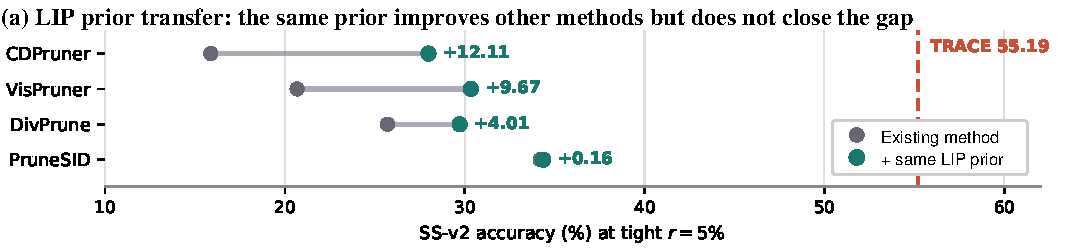
\includegraphics[width=0.95\linewidth]{figures/fig4_prior_transfer.pdf}\\[1pt]
    \vspace{-1mm}
    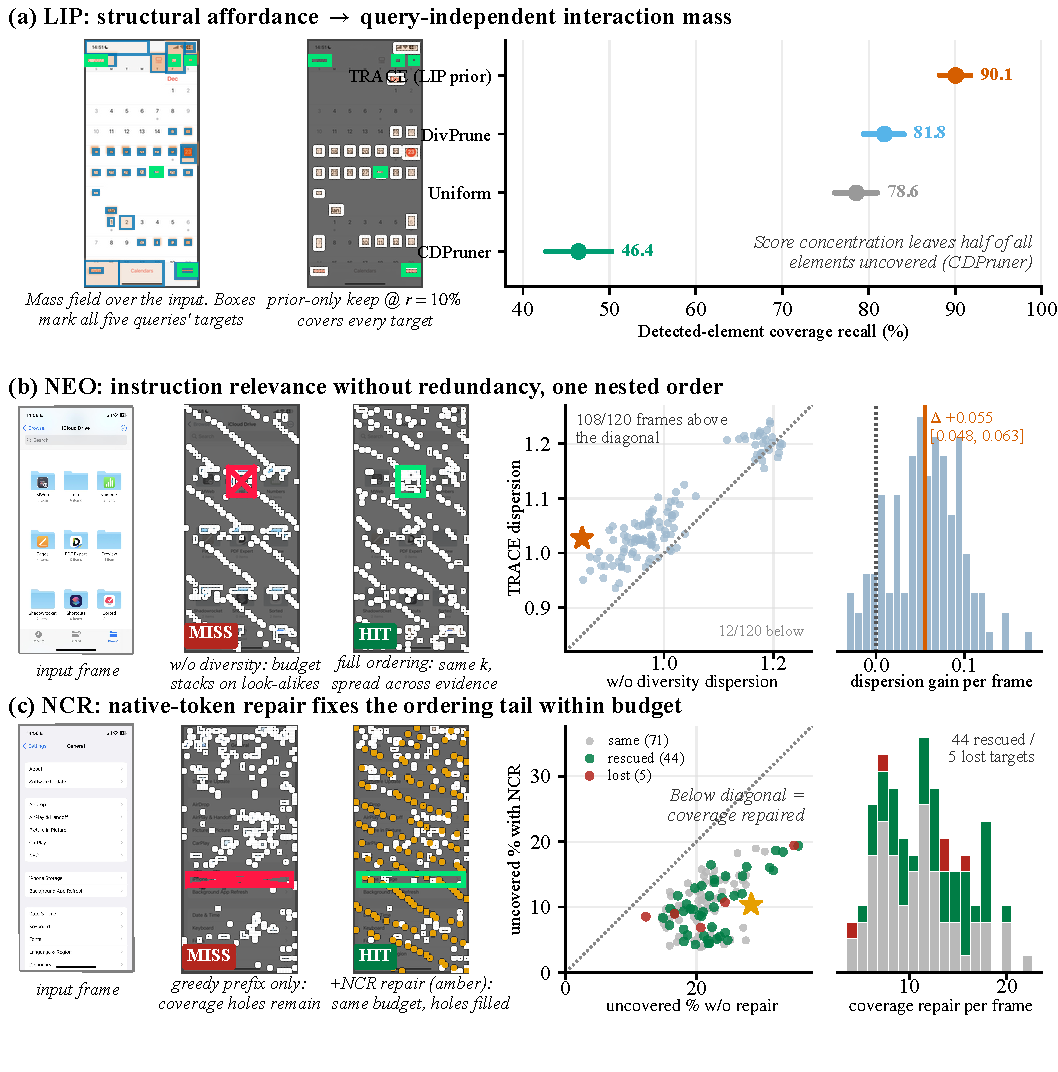
\includegraphics[width=0.95\linewidth, trim=0 0 0 176, clip]{figures/fig4_modules.pdf}
    \vspace{-3mm}
    \caption{Mechanism validation with \textbf{GUI-Owl-1.5-8B} on SS-v2. 
    %
    (a)~Analysis of the \lmp{} prior. 
    %
    (b)~Analysis of the \nwe{} diversity term. 
    %
    (c)~Analysis of the \awc{} coverage and target retention.}
    \label{fig:modules}
    \vspace{-3.5mm}
    \end{figure}
    \begin{figure}[t]
        \centering
        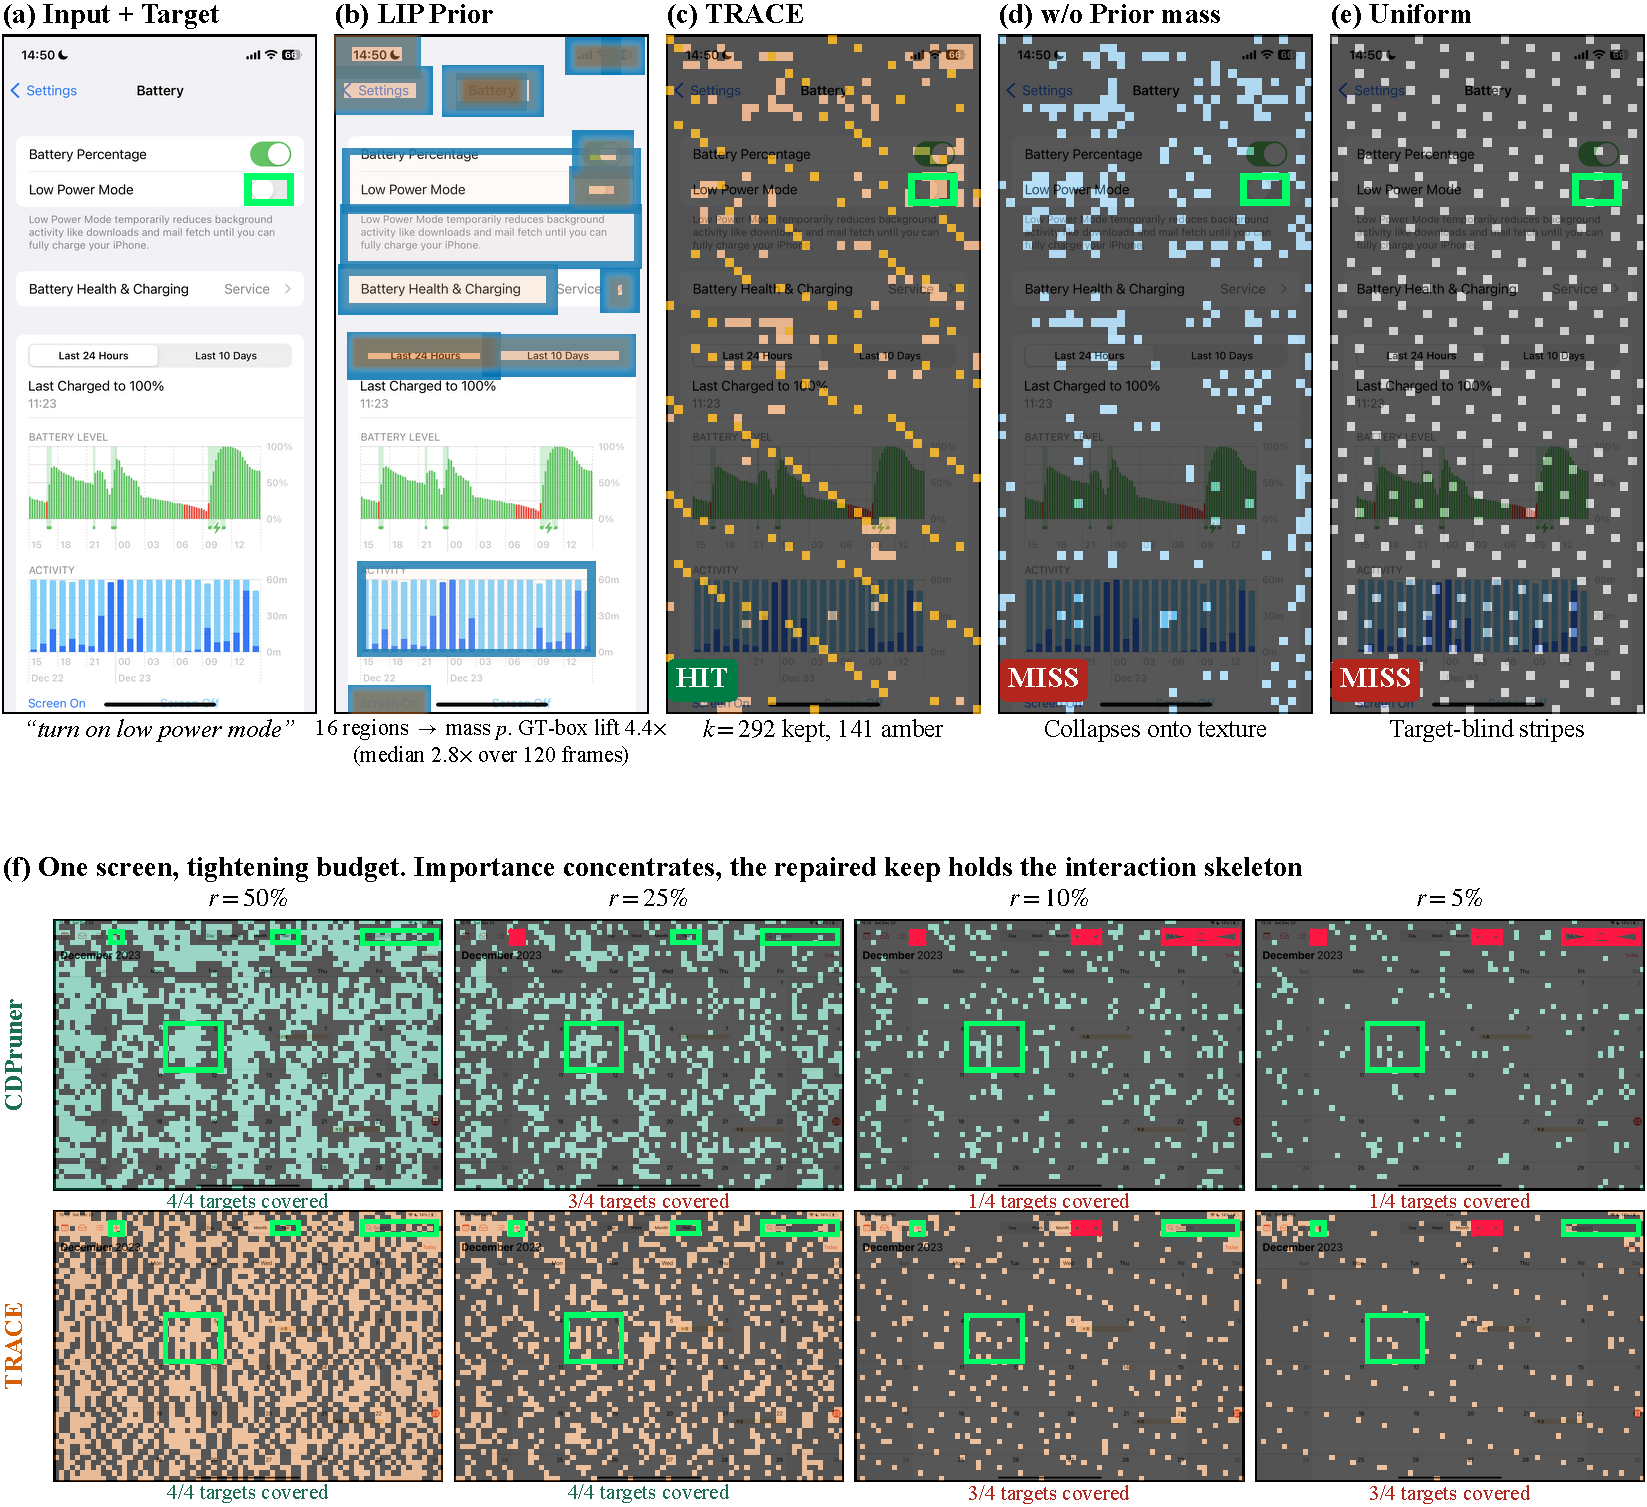
\includegraphics[width=0.95\linewidth, trim=0 0 0 426, clip]{figures/fig5_keepmaps.pdf}
        \vspace{-3.5mm}
        \caption{Keep maps on one SS-v2 screen carrying four instruction targets with \textbf{GUI-Owl-1.5-8B}.}
        \label{fig:keep-maps}
        \vspace{-2mm}
    \end{figure}
\subsection{Ablation Studies}
\label{sec:exp-ablation}
\label{sec:exp-modules}
\label{sec:exp-mech}
\label{sec:exp-analysis}
\label{sec:exp-transfer}
\label{sec:exp-eff}
\noindent\textbf{Analysis of Key Modules.}
As shown in Tab.~\ref{tab:ablation-main}, we analyze the contribution of each module in \method{}.
%
On SS-v2 at $\keepr{=}10\%$, the prior scored by top-$k$ reaches $32.63\%$ and \nwe{} alone reaches $36.48\%$.
%
In contrast, combining the two stages reaches $56.45\%$, which is \textbf{19.97\%} higher than either stage alone.
%
Adding \awc{} then raises SS-v2 accuracy from $56.45\%$ to $73.90\%$ and lifts tight Mind2Web from $27.79\%$ to $34.20\%$.
%
The prior thus locates operable regions, and the residual ordering keeps redundant tokens from consuming the budget.
%
Finally, \awc{} restores the spatial coverage lost to importance concentration.
%
These results fully verify the effectiveness of each module.
\\
\noindent\textbf{Module Design Choices.}
We further evaluate the design choices inside each module.
%
\noindent\textit{(1) Scoring factors inside \nwe{}.}
As shown in Tab.~\ref{tab:ablation-neo}, removing any one scoring factor degrades accuracy on all four benchmarks. 
%
Specifically, removing the prior costs the most, up to $-23.74\%$ on SS-v2. 
%
These results verify the complementarity of the three factors.
%
\noindent\textit{(2) Ordering form inside \nwe{}.}
As shown in Tab.~\ref{tab:ablation-neoform}, doubling the likelihood weight, pooling the query by log-mean-exp or collapsing it to the mean row costs $3.61\%$--$10.53\%$ on the two grounding benchmarks. 
%
These results verify the importance of each choice in the ordering rule.
%
\noindent\textit{(3) Energy attributes inside \lmp{}.}
As shown in Tab.~\ref{tab:ablation-lip}, removing any single energy attribute lowers accuracy on both benchmarks. 
%
Among the attributes, containment and resonance contribute the most, while contrast and entropy contribute less.
%
\noindent\textit{(4) Repair rules inside \awc{}.}
As shown in Tab.~\ref{tab:ablation-ncr}, stride tokens outperform feature medoids on the current frame, reaching $67.92\%$ on SS-v2 and $37.63\%$ on SS-Pro while the medoids reach $58.65\%$ and $30.11\%$.
%
The preference reverses on the history frame, where stride tokens cost $1.40\%$ on OmniGUI.
%
Thus, we adopt the stride rule on the current frame and the medoid rule on the history frame.
\begin{figure}[t]
    \centering
    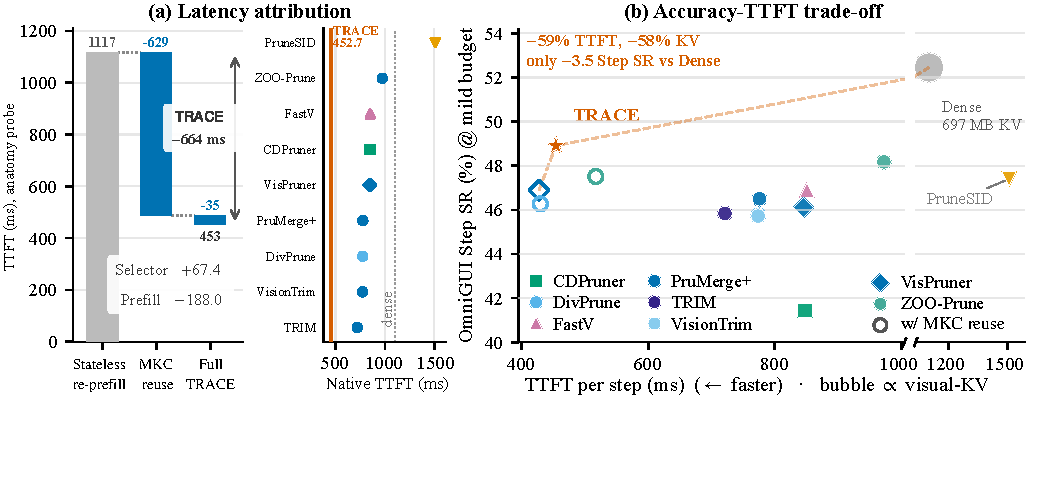
\includegraphics[width=1\linewidth]{figures/fig7_pareto.pdf}
    \vspace{-4mm}
    \caption{Serving efficiency analysis with \textbf{GUI-Owl-1.5-8B} on OmniGUI. 
    (a)~Latency attribution of the TTFT budget.
    %
    (b)~Accuracy--TTFT trade-off, where hollow markers denote existing methods ported onto the \kvr{} path and bubble area encodes the visual KV cache.}
    \label{fig:pareto}
    \vspace{-2mm}
\end{figure}
\\
\noindent\textbf{Mechanism Validation.}
\noindent\textit{(1) Prior transfer across methods.}
We graft the same interaction prior onto four existing methods at the tight budget. 
%
As shown in Fig.~\ref{fig:modules} (a), every method improves, by $+0.16\%$ to $+12.11\%$. However, the best reaches only $34.36\%$, still far below \method{}'s $55.19\%$. Moreover, the prior selected alone scores just $17.06\%$.
%
The margin therefore comes from converting the layout signal into a nested and coverage-aware order rather than from the detector itself.
%
\noindent\textit{(2) Dispersion under the diversity term.}
As shown in Fig.~\ref{fig:modules} (b), without the \nwe{} diversity term, the order spends its budget on repeated glyphs. By comparison, the full ordering spreads the keep more widely on GUI screenshots.
%
\noindent\textit{(3) Target rescue under coverage repair.}
As shown in Fig.~\ref{fig:modules} (c), \awc{} reduces the uncovered targets on most frames at the same budget. In turn, this repair rescues the target on $44$ frames while losing it on only $5$.
%
These results verify the mechanism of each module.
\\
\noindent\textbf{Generalization across Backbones.}
We evaluate \method{} on UI-TARS-1.5-7B for generalization across model families.
%
As shown in Tab.~\ref{tab:uitars-transfer}, \method{} achieves the best performance at both budgets. 
%
Moreover, its margins over DivPrune grow from $0.39\%$--$2.80\%$ at the mild budget to $0.79\%$--$4.92\%$ at the tight budget.
%
The gap is again widest on tight Mind2Web, where \method{} reaches $17.92\%$ and DivPrune reaches $13.00\%$.
%
These gains fully demonstrate the generalization ability of \method{}.
\\
\noindent\textbf{Efficiency Analysis.}
\noindent\textit{(1) End-to-end serving result.}
We analyze the serving efficiency of \method{} with one CUDA-synchronized GPU.
%
As shown in Fig.~\ref{fig:pareto} (a), \method{} reduces TTFT from $1116.8$\,ms to $452.7$\,ms and the visual KV cache from $697$\,MB to $292$\,MB.
%
The pixel-input detector runs concurrently with the vision encode, so this measurement already charges the full critical-path selection cost.
%
Overall, \method{} is \textbf{2.4$\times$} faster than dense re-prefill and attains the highest Step~SR among existing pruning methods.
%
\noindent\textit{(2) Attribution of the gain.}
Fig.~\ref{fig:pareto} (a) further attributes this gain, where applying \kvr{} alone lowers TTFT from $1116.8$\,ms to $487.4$\,ms at unchanged accuracy.
%
Adding the complete selector then lowers TTFT further, to $452.7$\,ms at the mild budget and $397.8$\,ms at the tight budget.
%
Specifically, pruning cuts the remaining LLM prefill from $328.6$ to $140.6$ and $101.9$\,ms, which repays the $67.4$/$47.0$\,ms selection cost several times over.
%
As shown in Fig.~\ref{fig:pareto} (b), porting DivPrune, VisPruner and ZOO-Prune onto the same \kvr{} path improves their TTFT by $1.8$--$2.0\times$.
%
Even after this acceleration, all three methods still lag behind \method{}.
%
The \kvr{} path therefore supplies the largest saving, whereas the admitted order adds a second saving and the accuracy margin.
%
\noindent\textit{(3) Window truncation as an alternative.}
Keeping fewer dense frames is the non-selective alternative.
%
However, three recent frames still spend $90\%$ of the dense budget, and one frame still costs $1.66\times$ ours.
%
Thus, window truncation still leaves latency and memory usage high without accuracy gain.
